% !TEX root = ./sum1.tex
\section{Deterministic Model}

\subsection{Obtain Minimum Number of Rows to Cover Demand}

We are given a demand, for example, $(d_1, d_2, d_3, d_4, d_5, d_6) = (3,5,7,0,10,6)$, where $d_i$ indicates the number of group containing $i$ people. Suppose each group has to leave a seat to maintain social distancing with the adjacent groups. Regard the groups as items in the CSP, and rows as stocks to be cut.
With considering the social distancing, the size of each group should be treated as the actual size plus one. Then each row of seats should also add a dummy(virtual) seat for the same reason, and the number of all seats in each row is called the length of the row.

To find the minimum number of rows to satisfy the demand, we can formulate this problem as a cutting stock problem form and use the column generation method to obtain an approximate solution.

Similar to the concept of pattern in the CSP, let the $k$-th placing pattern of a line of seats with length $S$ into some of the $m$ group types be denoted as a vector $(t^k_1,t^k_2,\ldots,t^k_m)$. Here, $t^k_i$ represents the number of times group type $i$ is placed in the $k$-th placing pattern. For a pattern $(t^k_1,t^k_2,\ldots,t^k_m)$ to be feasible, it must satisfy: $\sum_{i=1}^m t^k_i s_i \leq S$, where $s_i$ is the size of group type $i$. Denote by $K$ the current number of placing patterns.


This problem is to decide how to place a total number of group type $i$ at least $g_i$ times, from all the available placing patterns, so that the total number of rows of seats used is minimized.

Immediately we have the master problem:

\[\begin{split}\mbox{min}\quad & \sum_{k \in K}^K x_{k}\\
 \mbox{s.t.} \quad & \sum_{k \in K}^K t_i^k x_k \geq d_i  \quad  \mbox{ for } i=1,\ldots,m \\
  & x_k \geq 0, \mbox{integer}\quad \mbox{for}~ k \in K,\ldots,K.\\
\end{split}\]

If $K$ includes all possible patterns, we can obtain the optimal solution by solving the corresponding IP. But it is clear that the patterns will be numerous, considering all possible patterns will be time-consuming.

Thus, we need to consider the linear relaxation of the master problem, and the optimal dual variable vector $\lambda$. Using $\lambda$ as the value assigned to each group type $i$, the next problem is to find a feasible pattern $(y_1,y_2,\ldots,y_m)$ that maximizes the product of $\lambda$ and $y$.


Then the corresponding sub-problem is:
\[\begin{split}\mbox{max}\quad & \sum_{i=1}^m \lambda_i y_{i}\\
        \mbox{s.t.} \quad & \sum_{i=1}^m w_i y_i \leq S  \\
        & y_i \geq 0, \mbox{integer}\quad \mbox{for}~ i=1,\ldots,m.\\
\end{split}\]

This is a knapsack problem, its solution will be used as an additional pattern in the master problem.
We should continue to add new pattern until all reduced costs are nonnegative. Then we have an optimal solution to the original linear programming problem.

But note that column generation method cannot gaurantee an optimal solution. If we want to reach the optimal solution, we should tackle with the integer formulation.

\begin{equation}
\begin{aligned}
\min \sum_{k \in K}^{K} y_{k} & \\
\sum_{k=1}^{K} x_{i k} & \geq d_{i} \quad i=1, \ldots, n \\
\sum_{i=1}^{n} a_{i} x_{i k} & \leq S y_{k} \quad k=1, \ldots, K \\
y_{k} & \in\{0,1\} \quad k=1, \ldots, K \\
x_{i k} & \geq 0 \text { and integer } i=1, \ldots, n ; k=1, \ldots, K
\end{aligned}
\end{equation}

$y_k =1$ if line $k$ is used and 0 otherwise, $x_{ik}$ is the number of times group $i$ is placed in row $k$, and $K$ is the upper bound on the number of the rows needed.

\subsection{Provide The Maximal Supply When Given Rows}\label{maximal_supply}

Let us review this problem in another way. In most cases where the number of rows is fixed, we hope to accommodate as many as people possible. That is, we should minimize the space loss.

% This can be illustrated from the following picture.
%
% \begin{figure}[h]%%图
% 	\centering  %插入的图片居中表示
% 	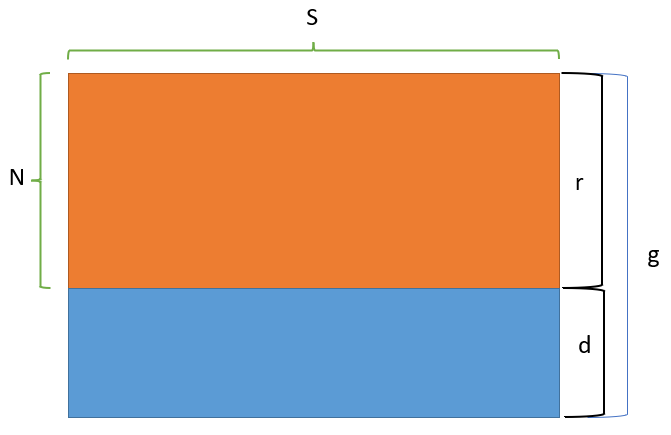
\includegraphics[width = 0.6\textwidth]{Figures/illu.png}  %插入的图,包括JPG,PNG,PDF,EPS等,放在源文件目录下
% 	\caption{The illustration for minimizing space loss}  %图片的名称
% 	\label{fig:illustration}   %标签,用作引用
% \end{figure}
%
% $N$: the number of given rows. $S$: the length of the line. $g$: total demand. $r$: remaining demand  $d$: discarded demand.

Then minimizing $NS - \sum_{i=1}^m r_i(s_i-1)$ equals to maximize $\sum_{i=1}^m r_i(s_i-1)$ and maximze $\sum_{i=1}^m (g_i - d_i)(s_i-1)$.

Notice that $\sum_{k=1}^K t_i^k x_k + d_i = g_i$, by substituting this equation we can obtain the objective function of the following master problem.

\begin{align}
(D) \quad \mbox{max}\quad & \sum_{k=1}^K(\sum_{i=1}^m (s_i-1)t_i^k) x_{k} \notag \\
\mbox{s.t.} \quad & \sum_{k=1}^K x_{k} \leq N \label{lambda1} \\
& \sum_{k=1}^K t_i^k x_k \leq g_i,\quad i=1,\ldots,m  \label{mu1} \\
& x_{k} \geq 0, \quad k = 1,\ldots,K \notag
\end{align}

Similarly, we consider the linear relaxation of the master problem and the optimal dual variable vector $\lambda,\mu$. Using $\lambda$ as the value assigned to the first constraint \eqref{lambda1} and $\mu$ to the second constraints \eqref{mu1}. This master problem is to find a feasible pattern $(t_1^{k_0},t_2^{k_0},\ldots, t_m^{k_0})$ that maximizes the reduced cost. The corresponding reduced cost is $c_{k_0} - c_B B^{-1}A_{k_0}$, where $c_{k_0} = \sum_{i=1}^m (s_i-1)t_i^{k_0}, c_B B^{-1} = (\lambda,\mu)$, $A_{k_0} = (1,t_1^{k_0},t_2^{k_0},\ldots,t_m^{k_0})^T$.
Use $y_i$ indicate the feasible pattern instead of $t_i^{k_0}$, we can obtain the sub-problem:

\[\begin{split}\mbox{max}\quad & \sum_{i=1}^m \left[(s_i-1) -\mu_i\right] y_{i} - \lambda \\
      \mbox{s.t.} \quad & \sum_{i=1}^m s_i y_i \leq S  \\
      & y_i \geq 0, \mbox{integer}\quad \mbox{for}~ i=1,\ldots,m.\\
\end{split}\]

Use column generation to generate a new pattern until all reduced costs are negative.

And the IP formulation can be shown as below:

\begin{equation}
\begin{aligned}
\mbox{max}\quad & \sum_{j=1}^{m} \sum_{i=1}^n (s_i-1) x_{ij} \\
\mbox{s.t.} \quad & \sum_{i=1}^n s_i x_{ij} \leq S, \quad j=1,\ldots,m \\
& \sum_{j=1}^{m} x_{ij} \leq g_i ,\quad i=1,\ldots,n \\
& x_{ij} \geq 0 \mbox{ and integer}, \quad i=1,\ldots,n, j=1,\ldots,m \\
\end{aligned}
\end{equation}

$m$ indicates the number of rows. $x_{ij}$ indicates the number of group type $i$ placed in each row $j$.

% For the cutting stock problem, $\min LP \leq \min LP^r \leq \min IP \leq \min IP^r$.
For our new problem, the column generation will give the upper bound (LP relaxation) and lower bound (restricted IP). After obtaining the patterns with column generation, restricted LP equals LP relaxation, $LP^r = LP$, which provides an upper bound. Thus, we have the relation, $\max LP \geq \max LP^r \geq \max IP \geq \max IP^r$.

To obtain an optimal solution, we should implement branch and bound into column generation. This method is called branch-and-price.

\subsection{Branch And Price}
Rather than solving IP directly to obtain the optimal integer solution, the commonly used method is to branch the fractional solution.

General branch is commonly as follows:
$\sum_{k \in K\left(k^{j}\right)} x_{k} = \alpha$, where $K(p) = \{k \in K: k\geq p\}$ (column subsets) for $p \in Z^m_+$, $\alpha$ is fractional.
$K = \{k \in N^m: \sum_{i=1}^m s_i k_i \leq S\}$ indicate all feasible patterns, and $x_k$ is the number of times pattern $k$ selected.
Given a feasible solution $x^*$ of LP that is not integral, take $k^*$ to be any maximal element of the set $\{k \in K: x_k^* \notin Z_+\}$. Then the only fractional term in this sum $\sum_{k \in K\left(k^{j}\right)} x_{k}^*$ is $x_{k^*}^*$.
Maximal means that the space left after cutting this pattern is less than the smallest size of the group.

Then the generic branching constraints will be:
$\sum_{k \in K(k^j)} x_{k} \leq U^{j}, \forall j \in G^u$ and $\sum_{k \in K(k^j)} x_{k} \geq L^{j}, \forall j \in H^u$, where $G^u$ and $H^u$ are sets of branching constraints of the form
\begin{equation}
 \sum_{k \in {K(k)}} x_{k} \leq\lfloor\alpha\rfloor
\end{equation} and
\begin{equation}
\sum_{k \in {K(k)}} x_{k} \geq \lceil\alpha\rceil
\end{equation}, respectively.

If we can always generate the maximal pattern, then any fractional column defines a branching set which contains only one member.

The corresponding restricted master problem will be reformulated as:

\[\begin{split}\mbox{max}\quad & \sum_{k\in K}(\sum_{i=1}^m (s_i-1)t_i^k) x_{k}\\
\mbox{s.t.} \quad & \sum_{k \in K} x_{k} \leq N \\
& \sum_{k \in K} t_i^k x_k \leq g_i,\quad i=1,\ldots,m\\
& \sum_{k \in K(k^j)} x_{k} \leq U^{j}, \forall j \in G^u \\
& \sum_{k \in K(k^j)} x_{k} \geq L^{j}, \forall j \in H^u \\
& x_{k} \geq 0, \quad k \in K
\end{split}\]

Let $(\pi,\lambda,\mu,v)$ be optimal dual variables associated with the added constraints.
The pricing problem(sub-problem) is:
\[\begin{split}\mbox{max}\quad & \left[(s_i-1) -\lambda_i\right] y_{i}- \pi - \sum_{j\in G^u}\mu_j z^j - \sum_{j\in H^u}v_j z^j \\
\mbox{s.t.} \quad & \sum_{i=1}^m s_i y_i \leq S  \\
& z^j =1 \mbox{ if } y \geq k^j; z^j =0 \mbox{ otherwise}  \\
& y_i \geq 0, \mbox{integer}\quad \mbox{for}~ i=1,\ldots,m.
\end{split}\]
$Y_k = \{(y,z): z=1,\text{ if } y \geq k,z=0 \text{ otherwise} \}$ can be formulated as MIPs.

The pricing problem is only affected when an upper bound has been placed on the value of the variable associated with the selected pattern. Because this variable could be a nonbasic variable for the LP. In this case, we have avoid regenerating this maximal pattern. Thus, we should solve a knapsack problem with a forbidden pattern set. Besides, the drawback of this method will be that the branch is unbalanced.

The procedure of branch and price is as follows:

\begin{itemize}
  \item [1)] Solve the restricted master problem with the initial columns.
  \item [2)] Use the pricing problem to generate columns.
  \item [3)] When the column generation method terminates, is the solution integral?

  Yes, update lower bound.

  No, update upper bound. And fathom node or branch to create two nodes.

  \item [4)] Select the next node until all nodes are explored.
\end{itemize}


\subsection{Occupancy}

For each pattern $k$, we use $\alpha_k, \beta_k$ to indicate the number of groups and the left space, respectively. Denote $(\alpha_k + \beta_k)$ as the loss for pattern k, $l(k)$.

For any pattern $k$, the occupancy is $\frac{S-l(k)}{S-1}$ and the largest occupancy is $\frac{S-l(k)}{S-1}, k \in I_1$. Thus, the largest occupancy for
multiple rows is also $\frac{S-l(k)}{S-1}, k \in I_1$ when all rows are largest patterns. $l(k)$ can be represented in another way, then we have the following lemma.

\begin{lem}
Suppose the size of group types be $s = [2,3,\ldots,u]$, the largest occupancy will be $\frac{S-q-\sign(r)}{S-1}$, where $q = \lfloor \frac{S}{u} \rfloor$, $\sign(r)=1$ if $r >0$, $\sign(r)=0$ if $r =0$.
\end{lem}

Suppose the size of group types be $s = [2,3,\ldots,u]$, the maximal group size be $u$ and $S = u\cdot q + r$. When $r =0$, the minimal loss is $q$, the largest occupancy will be $\frac{S-q}{S-1}$.
When $r>0$, the minimal loss will be $q+1$, the largest occupancy will be $\frac{S-q-1}{S-1}$.
Thus, the largest occupancy will be $\frac{S-q-\sign(r)}{S-1}$, where $q = \lfloor \frac{S}{u} \rfloor$, $\sign(r)=1$ if $r >0$, $\sign(r)=0$ if $r =0$.

% $S \equiv r \Mod{u}$

If we want the largest occupancy is no more than $\frac{1}{2}$, we have $\frac{S-\lfloor \frac{S}{u} \rfloor -1}{S-1} \leq \frac{1}{2} \Rightarrow \frac{S-1}{2} \leq \lfloor \frac{S}{u} \rfloor$. It is clear that when $u =2$ this inequality holds. When $u =3$, $S$ should be no larger than 3. In other cases, this inequality doesnot hold.

When $uq \leq S \leq uq + (u-1)$, $\lfloor \frac{S}{u} \rfloor$ equals $q$ and this ratio $\frac{S-q-1}{S-1}$ increases in $S$ when $q$ is fixed. Thus, when $S = uq + (u-1)$, the occupancy can reach maximum value, $\frac{S-q-1}{S-1}$.

When the social distancing is $2$, the size of group types will be $s = [3,4,\ldots,u]$, the occupancy will be $\frac{S-1-2*\lfloor \frac{S}{u} \rfloor}{S-1}$


2): The initial analysis about the loss between group type [2,3,\ldots,t-1] and [2,3,\ldots,t].
Suppose that $S \div t = q \ldots r$, then $S \div (t-1) = q \ldots q+r$
If $q+r < t-1$, the loss of the largest pattern for group size $t,(t-1)$, will be the same.
If $q+r = t-1$, $S = (t-1)* (q+1)$, the loss of the largest pattern for group size $t,(t-1)$, will be the same.

In other cases, the quotient of $S/(t-1)$ will be larger than that of $S/t$.
If the loss of the largest pattern for group size $(t-1)$ is $l$, the loss of the largest pattern for group size $t$ will be $l+1$.

3): If the size of group types is $s = [2,3,4]$, then we can obtain an optimal solution by the following way.

Suppose the demands for each group type are positive and $d_2,d_3,d_4$, respectively. The number of seats for each row is $S$. We have $N$ rows at the beginning. Let $S = 4 \times q +r, q = \lfloor \frac{S}{4} \rfloor$.

If $r = 0$, the largest pattern will be $(4,4,\ldots,4)$;

If $r = 1$, the largest pattern will be $(4,4,\ldots,4,3,2)$;

If $r = 2$, the largest pattern will be $(4,4,\ldots,4,2)$;

If $r = 3$, the largest pattern will be $(4,4,\ldots,4,3)$;

Repeat to generate the largest pattern until we do not have enough demands.
If any one of demands for group types runs out, the problem is reduced to the case of two group types, use the above method to solve this case.

Now suppose the rest demands are $d_2^{'},d_3^{'},d_4^{'}$ after deducting the demands of the largest patterns. Let $p = \lfloor \frac{d_4}{q} \rfloor$, then $d_4^{'} = d_4 - p \times q$. $p$ is equal to the number of rows where we placed groups.

$d_4^{'}$ should be less than $q$, otherwise, we can continue to generate the largest pattern.

For the next row, we place all rest $d_4^{'}$ groups with size of 4. Then we will have $S^{'} = S - d_4^{'} \times 4$ empty seats. The problem can be reduced to the case of two group types. That is, place groups with size of 3 as many as possible, the rest seats can be taken by group with size of 2.

For the rest $(N-p-1)$ rows, this problem is reduced to the case of two group types.

Extension: If the size of group types is $s = [2,3,u]$, $u$ is an integer and larger than 3, then we can obtain an optimal solution by the same way.

Remark: We can only obtain one optimal assignment, but this problem still has other optimal assignments.


% 4) Counter example: [6, 10, 15]*(4,2,1) under 30 seats.
%
% One row will be taken by one 15-size group and one 10-size group.
% Another one will be taken by one 10-size group and three 6-size groups.
%
% [4, 6, 9, 10]* (1, 2, 1, 1) under 18 seats.
%
% From the counter example, we can construct a case which has the positive demands for $[2,3,\ldots,10]$.
%
% When $d_4,d_5,d_6$ are all large for $[2,3,4,5,6]$, we can continue the above way to generate the largest pattern.
% That is the counter example of column generation not the policy.


% \begin{algorithm}[H]\label{algo2}
% \caption{The algorithm to construct an optimal solution for $[2,3,u]$}
% \begin{description}
%   \item[Step 1.] .
%   \vspace{10pt}
%   \item[Step 2.] .
% 	\vspace{10pt}
%   \item[Step 3.] .
%   \item[Step 4.] .
%   \item[Step 5.] .
% \end{description}
% \end{algorithm}

% Remaining questions:
%
% 1. In which situation, we can always satisfy the largest group size.
%
% (3,3,3,2,2) if the optimal pattern is (3,3,2,2). In this way, we will reject 3.
%
% 2. When S is small we will have a counter example easily. When S is large we are able to satisfy. the relation between S and u?
%
% 3. the number of maximal group size is equal to the number of rows.
% For example, for [2,3,4], if we have N groups of 4.

\subsection{Stochastic demands situation}

\subsubsection{Deterministic equivalent form}

Consider the decision maker who has to act in two consecutive stages. The first stage involves the choice of cutting patterns denoted by decision vector $\mathbf{x}$. At the second stage, some new information about demands is obtained, then a new vector $\mathbf{y}$ of decisions is to be chosen.

$\mathbf{x} \in \mathbb{Z}_{+}^{n}$ is the vector of first-stage scenario-independent decision variables, each component $x_k$ stands for the pattern $k$.

Use $\omega$ to index the different scenarios, each scenario $\omega \in \Omega, \Omega=\{1,2,\ldots,S\}$ corresponds to a particular realization of the demand vector, $\mathbf{D}_s = (d_{1s},d_{2s},\ldots,d_{ms})$.

$\mathbf{y} \in \mathbb{Z}_{+}^{m}$ is the vector of second-stage scenario-dependent decision variables, which include the number of holding groups, $y_{i \omega}^{+}$, when the supply overestimates the actual demand and the number of short groups, $y_{i \omega}^{-}$, when the supply understimates the actual demand for group type $i$ in scenario $\omega$.


Regarding the nature of the obtained information, we assume that there are $S$ possible scenarios, and that the true scenario is only revealed after $\mathbf{x}$ is chosen. 

Let $p_{\omega}$ denote the probability of any scenario $\omega$, which we assume to be positive.

We use the same definition as above, the size of group type $i$, $s_i$; the current pattern set, $K$; some pattern $k \in K$; the number of times that group type $i$ appears in pattern $k$, $t_{i}^k$.


The assignment will be determined before the realization of the random demand, here-and-now policy.


Considering that the seats assigned to some group type can be taken by the smaller group type, we assume that the holding group type $i$ can be utilized by the smaller group type $j = i-1$. Then we have the following scenario-based optimization problem:

\begin{equation}\label{deterministic_form}
\begin{aligned}
\max \quad & E_{\omega}\left[\sum_{i=1}^{m-1} (s_i-1) (\sum_{k \in K} t_i^k x_{k} + y_{i+1,\omega}^{+} - y_{i \omega}^{+}) + (s_m-1) (\sum_{k \in K} t_m^k x_{k} - y_{m \omega}^{+})\right] \\
\text {s.t.} \quad & \sum_{k \in K} t_{i}^{k} x_{k}-y_{i \omega}^{+}+
y_{i+1, \omega}^{+} + y_{i \omega}^{-}=d_{i \omega}, \quad i =1,\ldots,m-1, \omega \in \Omega \\
& \sum_{k \in K} t_{i}^{k} x_{k}-y_{i \omega}^{+}+y_{i \omega}^{-}=d_{i \omega}, \quad i = m, \omega \in \Omega \\
& \sum_{k \in K} x_{k} = N \\
& y_{i \omega}^{+} \cdot y_{i \omega}^{-}=0, \quad i \in I, \omega \in \Omega \\
& y_{i \omega}^{+}, y_{i \omega}^{-} \in \mathbb{Z}_{+}, \quad i \in I, \omega \in \Omega \\
& x_{k} \in \mathbb{Z}_{+}, \quad k \in K.
\end{aligned}
\end{equation}

The objective function contains two parts, the number of the largest group size that can be accommodated is $\sum_{k \in K} t_m^k x_{k} - y_{m \omega}^{+}$. The number of group size $i$ that can be accommodated is $\sum_{k \in K} t_i^k x_{k} + y_{i+1,\omega}^{+} - y_{i \omega}^{+}$.

Reformulate the objective function,

\begin{align*}
  & E[\sum_{i=1}^{m-1} (s_i-1) (\sum_{k \in K} t_i^k x_{k} + y_{i+1,\omega}^{+} - y_{i \omega}^{+}) + (s_m-1) (\sum_{k \in K} t_m^k x_{k} - y_{m \omega}^{+})] \\
  =& \sum_{k \in K}(\sum_{i=1}^m (s_i-1)t_i^k) x_{k}- \sum_{\omega =1}^{S} p_{\omega} \left(\sum_{i=1}^{m}(s_i-1)y_{i \omega}^{+} - \sum_{i=1}^{m-1}(s_i-1)y_{i+1, \omega}^{+}\right) \\
  =& \sum_{k \in K}(\sum_{i=1}^m (s_i-1)t_i^k) x_{k} - 
  \sum_{\omega =1}^{S} p_{\omega} \left((s_1-1)y_{1 \omega}^{+} + \sum_{i=2}^{m}(s_{i}-s_{i-1}) y_{i \omega}^{+} \right)
\end{align*}

When $s_i = i+1$, the objective function is $\sum_{k \in K}(\sum_{i=1}^m i t_i^k) x_{k} - \sum_{\omega =1}^{S} p_{\omega} \sum_{i=1}^{m} y_{i \omega}^{+}$.


This programming is in a deterministic equivalent form. 
The linear constraints associated with scenarios can be written in a matrix form as
\[\mathbf{T} \mathbf{x} + \mathbf{V}_\omega \mathbf{y}_\omega = \mathbf{D}_\omega, \omega\in \Omega\]

Each column of $T$ represents a cutting pattern.
$\mathbf{V}_s = [\mathbf{W} ~ \mathbf{I}]$.  

$$
\mathbf{W}=\left[\begin{array}{ccccc}
-1 & 1 & \ldots & & 0 \\
& \ddots & \ddots & & \vdots \\
& & & & 1 \\
0 & & & & -1
\end{array}\right]_{m \times m}
$$

and $\mathbf{I}$ is the identity matrix.

$$
\mathbf{y}_{s}=\left[\begin{array}{l}
\mathbf{y}_{s}^{+} \\
\mathbf{y}_{s}^{-}
\end{array}\right], \quad s \in \Omega
$$

$\mathbf{y}_{s}^{+}=\left[\begin{array}{lllll}y_{1 s}^{+} & y_{2 s}^{+} & \cdots & y_{m s}^{+}\end{array}\right]^{T}, \mathbf{y}_{s}^{-}=\left[\begin{array}{llll}y_{1 s}^{-} & y_{2 s}^{-} & \cdots & y_{m s}^{-}\end{array}\right]^{T}$.

Thus, the linear constraints have the following structure:

$$
\left[\begin{array}{cccccccccc}
\mathbf{T} & \mathbf{W} & \mathbf{I} & & & & & & & \\
\mathbf{T} & & & \mathbf{W} & \mathbf{I} & & & & & \\
\mathbf{T} & & & & & \mathbf{W} & \mathbf{I} & & & \\
\vdots & & & & & & & \ddots & & \\
\mathbf{T} & & & & & & & & \mathbf{W} & \mathbf{I}
\end{array}\right],
$$

As we can find, this formulation is a large-scale problem even if the number of possible scenarios $K$ is moderate. Thus, we need to reformulate the problem and use a decomposition method.

Remark: This paper \cite{alem2010cutting} mentions that it is possible to set $y_1 =0$ by assuming the first scenario presents the largest probability. In this way, $x$ can be determined in an easy way. But we will not follow that.

\subsubsection{Two-stage stochastic programming}

Let $c_k = \sum_{i=1}^m (s_i-1)t_i^k$, $f{'}y_{\omega} = -\left((s_1-1)y_{1 \omega}^{+} + \sum_{i=2}^{m}(s_{i}-s_{i-1}) y_{i \omega}^{+}\right)$. The objective function of problem \eqref{deterministic_form} can be expressed as $c{'}x + \sum_{\omega} p_{\omega}f{'}y_{\omega}$.

Once $x$ is fixed, the optimal second stage decision $y_{\omega}$ can be determined by solving for each $\omega$ the following problem:

\begin{equation}\label{BD_sub}
\begin{aligned}
  \max \quad & f{'} y_{\omega} \\
  \text {s.t.} \quad & \mathbf{T}x + \mathbf{V} y_{\omega} = d_{\omega} \\
   & y_{\omega} \geq 0
\end{aligned}
\end{equation}


Let $z_{\omega}(x)$ be the optimal value of the problem \eqref{BD_sub}, together with the convention $z_{\omega}(x) = \infty$ if the problem is infeasible. 

Now go back to consider the optimization of $x$, we are faced with the problem:

\begin{equation}\label{BD_master}
  \begin{aligned}
    \max \quad & c{'} x + \sum_{\omega \in \Omega} p_{\omega} z_{\omega}(x) \\
    \text {s.t.} \quad & \sum_{k \in K} x_k = N \\
     & x \geq 0
  \end{aligned}
\end{equation}

In order to solve this problem, we should only consider those $x$ for which $z_{\omega}(x)$ are all finite. Notice that the feasible region of the dual of problem \eqref{BD_sub} does not depend on $x$. We can form its dual, which is 

\begin{equation}\label{BD_sub_dual}
  \begin{aligned}
    \min \quad & \alpha{'}_{\omega} (\mathbf{d}_{\omega}- \mathbf{T}x) \\
    \text {s.t.} \quad & \alpha{'}_{\omega} \mathbf{V} \geq f{'}
  \end{aligned}
  \end{equation}

Let $P = \{\alpha|\alpha{'}V \geq f{'}\}$. 
We assume that $P$ is nonempty and has at least one extreme point. Then, either the dual problem \eqref{BD_sub_dual} has an optimal solution and $z_{\omega}(x)$ is finite, or the primal problem \eqref{BD_sub} is infeasible and $z_{\omega}(x) = \infty$.  

Let $\mathcal{O}$ be the set of all extreme points of $P$ and $\mathcal{F}$ be the set of all extreme rays of $P$. Then $z_{\omega} > -\infty$ if and only if $(\alpha^{j}){'}(\mathbf{d}_{\omega}- \mathbf{T}x) \geq 0, \alpha^{j} \in \mathcal{F}$, which stands for the feasibility cut. 

\begin{thm}\label{feasible_region}
  The feasible region, P, is bounded. And the extreme points are all integral.
\end{thm}

\begin{pf}[Proof of theorem \ref{feasible_region}]
Notice that $V =(W,~I)$, $W$ is a totally unimodular matrix. Then, we have $\alpha{'}W \geq -\bar{s}, \alpha{'}I \geq 0$. Thus, the feasible region is bounded.
And $\bar{s}_i = s_i - s_{i-1}, s_0 =1$ are integral, so the extreme points are all integral.
\qed
\end{pf}

Remark: we only need to consider the optimality cut in the following decomposition method.

When $s_i = i+1$, $f{'} = [-\mathbf{1},~\mathbf{0}], V =(W,~I)$, we have $\alpha{'}W \geq -1, \alpha{'}I \geq 0$. Thus, it is easy to find that the feasible region is bounded, i.e., $P$ does not contain any extreme rays. Furthermore, let $\alpha_0 = 0$, then we have 
\begin{align*}
  & 0 \leq \alpha_1 \leq 1,\\ 
  & 0 \leq \alpha_2 \leq \alpha_1 + 1, \\
  & \cdots, \\
  & 0 \leq \alpha_m \leq \alpha_{m-1} + 1
\end{align*}

When $s_i$ is integral, we can still use the same way to obtain the dual optimal solution.

When we are given $x^{*}$, the demand that can be satisfied by the arrangement is $T x^{*} = d_0 = (d_{1,0},\ldots,d_{m,0})$.
Then plug them in the subproblem \eqref{BD_sub}, we can obtain the value of $y_{i \omega}$ recursively:
\begin{equation}\label{y_recursively}
\begin{aligned}
  & y_{m \omega}^{-}=\left(d_{m \omega}-d_{m 0}\right)^{+} \\
  & y_{m \omega}^{+}=\left(d_{m 0}-d_{m \omega}\right)^{+} \\
  & y_{i \omega}^{-}=\left(d_{i \omega}-d_{i 0} - y_{i+1, \omega}^{+} \right)^{+}, i =1,\ldots,m-1 \\
  & y_{i \omega}^{+}=\left(d_{i 0}- d_{i \omega} + y_{i+1, \omega}^{+}\right)^{+}, i =1,\ldots,m-1
\end{aligned}
\end{equation}

The optimal value for scenario $\omega$ can be obtained by $f{'} y_{\omega}$, then we need to find the dual optimal solution.


\begin{thm}\label{optimal_sol_sub_dual}
  An optimal solution to problem \eqref{BD_sub_dual} is given by 
\begin{equation}\label{BD_sub_simplified}
  \begin{aligned}
    & \alpha_{i \omega} =0, i =1,\ldots,m \quad \text{if}~  y_{i \omega}^{-} > 0   \\
    & \alpha_{i \omega} = \alpha_{i-1, \omega}+1, i =1,\ldots,m \quad \text{if}~ y_{i \omega}^{+} > 0
  \end{aligned}
\end{equation}
\end{thm}

When $y_{i \omega}^{+} = 0$ and $y_{i \omega}^{-} = 0$, $\left(d_{i 0}- d_{i \omega} + y_{i+1, \omega}^{+}\right) = 0$, $d_{i \omega}- d_{i 0} = y_{i+1, \omega}^{+} \geq 0$.

If $y_{i+1, \omega}^{+} > 0$, $\alpha_{i \omega} = 0$,
if $y_{i+1, \omega}^{+} = 0$, $0 \leq \alpha_{i \omega} \leq \alpha_{i-1, \omega} +1$.

\begin{pf}[Proof of theorem \ref{optimal_sol_sub_dual}]
  According to the complementary relaxation property, when
$d_{i \omega} > d_{i 0} \Rightarrow y_{i \omega}^{-} >0$, then $\alpha_{i \omega} =0$ for all $i$; when $d_{i \omega} < d_{i 0} \Rightarrow y_{i \omega}^{+} >0$, then $\alpha_{i \omega} = \alpha_{i-1,\omega} +1, i =1,\ldots,m$. 

When $d_{i \omega} = d_{i 0}$,  we can find that $\alpha_{i \omega} = \alpha_{i-1, \omega} + 1$ will minimize the objective function.

Let $\Delta d = d_{\omega} - d_0$, then the elements in $\Delta d$ will be negative integer, positive integer and zero. The value of $\alpha$ associated with zero will not affect objective function directly, only affect the value of $\alpha$ associated with negative integer. The larger the value of $\alpha$ associated with negative integer is, the smaller the objective function will be. Thus, let $\alpha_{i \omega} = \alpha_{i-1, \omega} + 1$ when $d_{i \omega} = d_{i 0}$ can obtain the minimized objective function.
\qed
\end{pf}

We can use the forward method, starting from $\alpha_{1 \omega}$ to $\alpha_{m \omega}$, to obtain the value of $\alpha_{\omega}$ rather than solving a linear programming.


We know that $z_{\omega}(x)$ is finite and it is the optimal value of the problem \eqref{BD_sub} and this value will be attained at extreme points of the set $P$. Thus, we have $z_{\omega}(x) = \min_{\alpha^j \in \mathcal{O}} (\alpha^{j}){'}(\mathbf{d}_{\omega}- \mathbf{T}x)$. 

\subsubsection{Benders decomposition}

Let $z_{\omega}(x)$ be the upper bound of $z_{\omega}$ such that $(\alpha^{j}){'}(\mathbf{d}_{\omega}- \mathbf{T}x) \geq z_{\omega}, \alpha^j \in \mathcal{O}$, which is the optimality cut.

Use the characterization of $z_{\omega}(x)$ in the problem 
\eqref{BD_master}, and take into account the optimality condition, we can conclude the master problem \eqref{BD_master} will have the form:

\begin{equation}\label{BD_master1}
  \begin{aligned}
    \max \quad & c{'} x + \sum_{\omega \in \Omega} p_{\omega} z_{\omega} \\
    \text {s.t.} \quad & \sum_{k \in K} x_k = N \\
    & (\alpha^{j}){'}(\mathbf{d}_{\omega}- \mathbf{T}x) \geq z_{\omega}, \alpha^j \in \mathcal{O}, \forall \omega \\
     & x \geq 0
  \end{aligned}
\end{equation}

Now use a small subset of $\mathcal{O}$, $\mathcal{O}^t$, to substitute the original one, then we have a relaxation of the master problem \eqref{BD_master1}:

\begin{equation}\label{BD_master2}
  \begin{aligned}
    \max \quad & c{'} x + \sum_{\omega \in \Omega} p_{\omega} z_{\omega} \\
    \text {s.t.} \quad & \sum_{k \in K} x_k = N \\
    & (\alpha^{j}){'}(\mathbf{d}_{\omega}- \mathbf{T}x) \geq z_{\omega}, \alpha^j \in \mathcal{O}^{t}, \forall \omega \\
     & x \geq 0
  \end{aligned}
\end{equation}


Given the initial $\mathcal{O}^{t}$, we can obtain the optimal $\mathbf{x}^{*}$ and $\mathbf{z}^{*}=(z^{*}_1,\ldots, z^{*}_S)$. We need to check whether $(\mathbf{x}^{*}, \mathbf{z}^{*})$ is also an optimal solution to the full master problem. 

\begin{lem}\label{one_ep_feasible}
When each scenario has at least any one optimality cut, the problem \eqref{BD_master2} is always bounded.
\end{lem}

\begin{pf}[Proof of lemma \ref{one_ep_feasible}]
  Suppose we have one extreme point $\alpha^{\omega}$ for each scenario. Then we have the following problem.
  \begin{equation}\label{lemma_eq}
    \begin{aligned}
      \max \quad & c{'} x + \sum_{\omega \in \Omega} p_{\omega} z_{\omega} \\
      \text {s.t.} \quad & \sum_{k \in K} x_k = N \\
      & (\alpha^{\omega}){'}\mathbf{d}_{\omega} \geq (\alpha^{\omega}){'} \mathbf{T}x + z_{\omega}, \forall \omega \\
       & x \geq 0
    \end{aligned}
  \end{equation}
  Problem \eqref{lemma_eq} reaches its maximum when $(\alpha^{\omega}){'}\mathbf{d}_{\omega} = (\alpha^{\omega}){'} \mathbf{T}x + z_{\omega}, \forall \omega$. Substitute $z_{\omega}$ with these equations, we have 
  \begin{equation}\label{lemma_eq2}
    \begin{aligned}
      \max \quad & c{'} x - \sum_{\omega}p_{\omega}(\alpha^{\omega}){'}Tx + \sum_{\omega} p_{\omega} (\alpha^{\omega}){'} \mathbf{d}_{\omega} \\
      \text {s.t.} \quad & \sum_{k \in K} x_k = N \\
      & x \geq 0
    \end{aligned}
  \end{equation}
  Notice that $x$ is bounded, then the problem \eqref{lemma_eq} is bounded. Adding more optimality cuts will not make the optimal value larger. Thus, the problem \eqref{BD_master2} is bounded. 
  \qed
\end{pf}


When some scenario only includes one optimality cut, we can substitute $z_{\omega}$ into the objective function. 

According to theorem \ref{optimal_sol_sub_dual}, we can obtain the optimal solution, $\alpha_{\omega}^{*}$, to problem \eqref{BD_sub_dual}. When $\mathbf{x}_0$ is given, $z_{\omega}^{0} = \alpha_{\omega}^{*}(d_{\omega} - T \mathbf{x}_0)$ will give a minimal upper bound of $z_{\omega}$, thus all the left constraints associated with other extreme points are redundant.

Notice that $(x_0, z_{\omega}^{0})$ is a feasible solution ($c{'} x_0 + \sum_{\omega \in \Omega} p_{\omega} z_{\omega}^{0}$ is the lower bound) when the extreme points are $\alpha_{\omega}$. The problem \eqref{lemma_eq} associated with $\alpha_{\omega}$ will give an optimal solution $(x_1, z_{\omega}^{1})$. (Upper bound)

\subsubsection{Column-and-cut generation}

Recall that $T$ is a subset of the set of all possible cutting patterns, thus we need to find more cutting patterns by the column generation.

\begin{lem}\label{full_cutting_pattern}
When the group sizes are consecutive integers starting from 2, i.e., $[2,3,\ldots,u]$, $T$ only need include the full or largest cutting patterns.
\end{lem}

We can always find a full pattern which accomodates more people than any non-full pattern except when the largest pattern is $(u, \ldots, u, 1)$.

Suppose that we have $p$ cuts during some iteration, let $(\pi=\left[\pi_{1}, \pi_{2},\cdots,\pi_{p}\right],\lambda)$ be optimal dual variables associated with the scenario constraints and row number constraint.

Then the pricing problem will be

\begin{equation}\label{add_cutting_pattern}
  \begin{aligned}
  \mbox{max}\quad & \sum_{i=1}^m \left[(s_i-1) -\sum_{p}\pi_{p}\alpha_{i}^{p} \right] y_{i} - \lambda \\
  \mbox{s.t.} \quad & \sum_{i=1}^m s_i y_i \leq L  \\
  & y_i \geq 0, \mbox{integer}\quad \mbox{for}~ i=1,\ldots,m
\end{aligned}
\end{equation}

where $y_i$ indicate the number of times group type $i$ placed in the new pattern.

By solving the pricing problem, we can obtain a new cutting pattern, then add it to $T$. Then solve the problem \eqref{BD_master2} to obtain $(x^{*}, z^{*})$ and continue the column-and-cut generation.

After we obtained $x_1$, add new optimality cuts and cutting patterns, then repeat the above procedure until the optimal value does not increase anymore.

The steps of the algorithm can be described as below,

\begin{algorithm}[H]\label{column_and_cut_algo}
  \caption{The column-and-cut generation algorithm}
    \begin{description}
    \item[Step 1.] Solve LP \eqref{lemma_eq} with all $\alpha_{\omega}^0 = \mathbf{0}$ for each scenario.
    Then, obtain the solution $(x_0, z_{\omega}^{0})$ and dual solution $(\pi, \lambda)$.

    \item[Step 2.] Set the upper bound $UB = c{'} x_0 + \sum_{\omega \in \Omega} p_{\omega} z_{\omega}^{0}$ 
    \item[Step 3.] 
    For $x_0$, we can obtain $\alpha_{\omega}^{1}$ and $z_{\omega}^{(0)}$ for each scenario, set the lower bound $LB = c{'} x_0 + \sum_{\omega \in \Omega} p_{\omega} z_{\omega}^{(0)}$
    % \item[Step 4.] Solve problem \eqref{BD_master2} with the scenario constraints, we can obtain a new solution $(x_1, z_{\omega}^{1})$ and dual solution $(\pi,\lambda)$. 
    
    % The optimal value must be no less than the value associated with $(x_0, z_0)$. If these values are equal, terminate this algorithm. 
    \item[Step 4.]
    If $(\alpha_{\omega}^{1}){'}(\mathbf{d}_{\omega}- \mathbf{T}x_0) < z_{\omega}^{(0)}$, add one new constraint, $(\alpha_{\omega}^{1}){'}(\mathbf{d}_{\omega}- \mathbf{T}x) \geq z_{\omega}$, to LP \eqref{BD_master2}.
    
    \item[Step 5.]
    Solve \eqref{add_cutting_pattern} with $(\pi,\lambda)$, add a new cutting pattern and update $\mathbf{T}$.
    \vspace{5pt}
    \item[Step 6.] Solve the updated LP \eqref{BD_master2}, obtain a new solution $(x_1, z_{\omega}^{1})$ and update UB.
    \item[Step 7.] Repeat step 3 until $|UB - LB| < \epsilon$.(Or in our case, UB converges.)
   \end{description}
  \end{algorithm}

Step 7, notice that $LB$ is monotone, but $UB$ is not monotone because $T$ will change.

Step 1 results from the lemma \ref{one_ep_feasible}.

After the algorithm terminates, we obtain the optimal $x^{*}$. The demand that can be satisfied by the arrangement is $T x^{*} = d_0 = (d_{1,0},\ldots,d_{m,0})$.
Then we can obtain the value of $y_{i \omega}$ from equation \eqref{y_recursively}.

\subsubsection{Results of the column-and-cut method}
% Suppose $S$ seats, group types are $\{2,\ldots,u\}$.
% $S = u \cdot q + r, r < u$.
% If we want to find all the full patterns, at first need to consider how to allocate $(u-r)$ seats.

% Let $d = u-r$, the results are showed below.

% Consider the number of different largest cutting patterns:

\begin{table}[ht]
  \begin{tabular}{l|l|l|l|l}
  \hline
  \# of scenarios number & \# of group types & \# of iterations & \# of cutting patterns & time(s) \\
  100  & 4  & 2 & 1 & 0.5 \\
  200  & 4  & 2 & 1 & 1 \\
  500  & 4  & 2 & 1 & 3 \\
  1000 & 4 & 2 & 1 & 5 \\
  2000 & 4 & 2 & 1 & 10 \\
  5000 & 4 & 2 & 1 & 24\\
  \hline
  \end{tabular}
\end{table}

The size of each row is 18.

Group types are $[2,3,4,5]$.

The scenarios are generated from $[5,15]$.

Given the number of rows is 3. The initial cutting pattern are gererated in the same way as before.

We can see that the number of cutting patterns and iterations is related with the size of row and group types.

The running time increases with the number of scenarios linearly.

Now Fix the number of scenarios at 500.

\begin{table}[ht]
  \begin{tabular}{l|l|l|l|l}
  \hline
  size of row & \# of group types & \# of iterations & \# of cutting patterns & time(s) \\
  10  & 4  & 1 & 0 & 0.8 \\
  20  & 4  & 3 & 0 & 3 \\
  30  & 4  & 4 & 2 & 6.3 \\
  40  & 4  & 5 & 1 & 9.6 \\
  50  & 4  & 7 & 3 & 16.5 \\
  90  & 4  & 5 & 1 & 9 \\
  100 & 4 & 1 & 0 & 1.29 \\
  200 & 4 & 1 & 0 & 1.26 \\
  500 & 4 & 1 & 0 & 1.25 \\
  \hline
  \end{tabular}
\end{table}

One interesting thing is that the running time are higher when the size of row is 50. Then we fix the size of row at 50, just change the number of group types. (Starting from 2 and group types are consecutive integers starting from 2)

\begin{table}[ht]
  \begin{tabular}{l|l|l|l|l}
  \hline
  \# of group types & size of row & \# of iterations & \# of cutting patterns & time(s) \\
  2  & 50  & 1 & 1 & 1.26 \\
  3  & 50  & 4 & 2 & 6.3 \\
  4  & 50  & 7 & 3 & 16.1 \\
  5  & 50  & 5 & 5 & 9.6 \\
  6  & 50  & 5 & 4 & 9.7 \\
  7  & 50  & 4 & 4 & 6.5 \\
  8  & 50 & 4 & 3 & 6.2 \\
  9  & 50 & 3 & 1 & 4 \\
  10 & 50 & 3 & 1 & 4.2 \\
  \hline
  \end{tabular}
\end{table}


% But the larger one can be divided into two smaller groups, $7 = 3 + 4$, still difficult to calculate the number of different full patterns.

% Example:
% $(2,2)$ will be inferior to $(1,3)$.
% $S =11, s =[2,3], p_1 =p_2 =0.5, N =3$.
% $T = 
%   \begin{pmatrix}
%   1 & 4  \\
%   3 & 1  
%   \end{pmatrix}$
% $x_{0} = 
% \begin{pmatrix}
% 2   \\
% 1  \end{pmatrix}$

% $d_0 = T x_{0} = \begin{pmatrix}
%   1 & 4  \\
%   3 & 1  
%   \end{pmatrix} \begin{pmatrix}
%     2   \\
%     1  \end{pmatrix} = \begin{pmatrix}
%       6   \\
%       7  \end{pmatrix}$

% $d_{1} = 
% \begin{pmatrix}
% 6   \\
% 6  \end{pmatrix}$ 
% $d_{2} = 
% \begin{pmatrix}
% 7   \\
% 7  \end{pmatrix}$
% $\Rightarrow  \alpha_{1} = (1,2),\alpha_{2} = (0,1).$

% Solve problem \eqref{lemma_eq2}, $x^{*} = (3,0){'}, z_{1} = 3, z_{2} = -2$.

% $d_0 = T x^{*} = \begin{pmatrix}
%     3   \\
%     9  \end{pmatrix}$
% $\Rightarrow  \alpha_{1}^{(1)} = (1,0),\alpha_{2}^{(1)} = (1,0).$

% $z_{1} = -3 <3$, add $\alpha_1^{(1)}$.

% \begin{equation}
%   \begin{aligned}
%     \max \quad & (7,6) (x_1,x_2){'} + \frac{1}{2} (z_1+z_2) \\
%     \text {s.t.} \quad & (0, 1)(6, 6){'} \geq (3,1) (x_1,x_2){'} + z_1 \\
%     & (2, 1)(6, 6){'} \geq (5,9) (x_1,x_2){'} + z_1 \\
%     & (0, 1)(7, 7){'} \geq (3,1) (x_1,x_2){'} + z_2 \\
%     & x_1 + x_2 = 3 \\
%     & x_1,x_2 \geq 0
%   \end{aligned}
% \end{equation}

% One observation is that if we can obtain the valid cuts every time, we only need to add at most $(K-1)$ cuts, where $K$ is the number of initial cutting patterns.




% For each $\omega$, if it satisfies $f{'} y_{\omega} < z^{*}_{\omega}$, then we have identified a violated constraint, $(\alpha^{t}){'}(\mathbf{d}_{\omega}- \mathbf{T}x^{*}) \geq z_{\omega}$, which can be added to the relaxed master problem. $\alpha^{t}$ is the dual optimal solution.
% If we have $(\alpha^{t(\omega)}){'}(\mathbf{d}_{\omega}- \mathbf{T}x^{*}) \geq z_{\omega}$ for all $\omega$, then we obtain $(\alpha^{t}){'}(\mathbf{d}_{\omega}- \mathbf{T}x^{*}) \geq z_{\omega}$. In this way, we have an optimal solution to the master problem \eqref{BD_master1} because no constraint is violated.


\subsubsection{Details about the initial cutting pattern}
It seems that the initial cutting patterns are not crucial to the complexity of the whole problem.

How to generate the initial cutting patterns depends on the demands for scenarios.

At least, we know that the full or largest patterns are needed.

\subsubsection{Complexity about the number of cutting patterns}
We only know that the full pattern will be used.

Demonstrate the number of cutting patterns is large.

The number of cutting patterns is equal to the number of solutions to $\sum_{i=1}^m s_i y_i = L$. $\{y_i\}$

\subsubsection{Two adjacent group types model}\label{sec_adjacent}
The model assumes two group types, group 1 and 2, with associated sizes $s_1 = s_2 + 1$.

It can help us accept or reject group 2 when the capacity of group 2 is not enough but the capacity of group 1 is sufficient.

Suppose that there are $x$ quantities of group 1 remaining and we receive a request from group 2.

If we accept the request, $(s_2 -1)$ people will be placed. If we reject it, we will place $x$ quantities of group 1 if and only if demand for group 1 is $x$ or higher. That is, if and only if $D_1 \geq x$. Thus, the expected number of people from reserving x units of capacity for group 1 is $(s_1-1)P(D_1 \geq x)$.

Therefore, we will accept a group 2 request if and only if $(s_{2}-1) \geq (s_{1}-1) P\left(D_{1} \geq x\right)
\Rightarrow P(D_1 < x) \geq \frac{1}{s_2}$.

If a continuous distribution $F(x)$ is used to model demand, $D_1$, then the optimal remaining capacity is given by the simpler expression, $x^{*} = F^{-1}(\frac{1}{s_2})$.

When we obtain the demand $d_0 = (d_0^2, d_0^3, d_0^4) = (6,7,8)$ from Algorithm 1.

The booking limits are 8 for group with size of 4, 15 for 3, 21 for 2.

\subsubsection{Scenario-based solution}

% \begin{algorithm}[H]\label{scenario_based}
%   \caption{The scenario-based method to deal with the dynamic situation}
%   \begin{description}
%     \item[Step 1.] We have several planning supplies, $d^{i} \in D$.
%     Let $d^{*} = \min_{i}\{d^{i}\}$
%     \vspace{5pt}
%     % \item[Step 2.] According to the patterns, arrange the arrival groups in one row as for as possible.
%     \item[Step 2.] Whenever some demand reaches $d^{*}_{i}+1$, we need to rebuild the scenarios according to the realized demands.
%     \item[Step 3.] If we have allocated a whole row, deduct the corresponding demands from the realized demands; if not, keep these demands(don't arrange the people with the seats) until we allocate a whole row.
%     \item[Step 4.] Set a stopping time; we will fix the patterns after that time. (The time can be determined when the number of planning demands is one or the number of remaining rows is small)
%     \item[Step 5.] When the corresponding demands run out, use the two-class model to judge whether we should accept the request.
%   \end{description}
% \end{algorithm}

\begin{algorithm}[H]\label{scenario_based}
  \caption{The scenario-based method to deal with the dynamic situation}
  \begin{description}
    \item[Step 1.] Obtain a linear solution from stochastic programming \eqref{BD_master1}.
    \item[Step 2.] If the linear solution(supply) is not integral, obtain several plannings.
    \item[Step 3.] Obtain the integral patterns from the integral supply.
    \item[Step 4.] Accept or reject group arrival according to the supply.
    \item[Step 5.] Update the scenario and the probability, add constraints when re-calculating stochastic programming.
    \item[Step 6.] Set a stopping time; we will fix the patterns after that time. (The time can be determined when the number of plannings is one or the capacity is small.)
    \item[Step 7.] Use DP or the several-class model to make the decision.
  \end{description}
\end{algorithm}

In step 5, we can update the scenarios whenever we accept the request or when some demand exceeds the supply then update the scenarios.

When we re-calculate the stochastic programming, we need to add the constraints, $(Tx)_{i} \geq a_{i}$, into \eqref{BD_master2}. $a_{i}$ is the number of group type $i$ we have accepted.

In step 7, choosing which method depends on what we know (demands distribution or arrival rates).

Initialization: suppose the planning supply is $[x_{1}, x_{2}, \ldots, x_{r}]$, then according to the capacity obtain its maximal number, $n_{i}^{*}, 1 \leq i \leq r$ when we only place one group type $i$.

For group type $i$, any scenarios with a larger number than $n_{i}^{*}$ will be merged into the scenario with $n_{i}^{*}$.
The corresponding probabilities will be $P_{i} = P(n = i), i < n_{1}^{*}, P_{n_{1}^{*}} = P(n \geq n_{1}^{*})$.

Every time we accept one group $i$, $n_{j}^{*}, j \neq i$ will change accordingly, and we can theoretically select the scenarios with the updated probability. 
But practically, we don't calculate it frequently when the capacity is enough at the beginning.


% When there come two groups with $2$ people, we accept them, then the maximal number of $3$ can only be $5$ right now. (Because we accepted two groups of $2$, the remaining capacity can only serve five groups with $3$ at most.) And the probability that the number of groups of $3$ is above five will be counted into five.


% Before realizing a whole row, we will keep these demands and don't let the customer take in the seats.

% 1. Why should we don't use the subset sum problem to decompose the whole problem, it will destroy global optimality. But notice that when we arrange row by row, it may also affect the optimality.

% Many symmetry structure/ Every step we need to solve a multiple knapsack problem(difficult).

% 3. Should we set a penalty if we reject some request?

\subsubsection{How to generate an integral demand from a fractional demand}

% Notice that the optimal linear solution only leaves one empty seat in the allocation. Thus, the fractional demand can be like $[6, 9\frac{1}{3}, 10, 14]$ or $[3, 7, 8\frac{1}{4}, 12]$ with corresponding group types $[2,3,4,5]$. ($\frac{1}{3} * 3 =1$)

If the optimal supply is $[2, 3.75, 4.25, 6.75]$, how should we deal with it?

\begin{thm}
An optimal integral supply can be derived from the fractional supply obtained by stochastic programming.
\end{thm}

% \begin{pf}[Proof]
% Suppose that an optimal supply obtained from stochatic programming, $[d_1,\ldots,d_{m-1},d_{m}]$, including several fractional elements, $d_{m-1}, d_{m}$.

% Recall that the objective function includes two parts, $Tx$ and $p_{\omega} \sum_{i}y_{i\omega}^{+}$.

% If we let $d_{m} \to \lceil d_{m} \rceil$($\lceil d_{m} \rceil - d_{m} = \alpha$), and take the short capacity from $d_{m-1}$. $(Tx)_{m}$ increases $\alpha$, $(Tx)_{m-1}$ decreases $\frac{m+1}{m} \alpha$, then $Tx$ part will increase $\frac{\alpha}{m}$.

% If $y_{m\omega}^{+} >0$, $(Tx)_{m} \nearrow$, $y_{m\omega}^{+} \nearrow$, $(Tx)_{m-1}-y_{m-1,\omega}^{+} \searrow$.
% The change of $y_{m\omega}^{+}$ will affect $y_{i\omega}^{+}, i< m$ correspondingly.

% % The $y_{i}$ part will increase $\frac{n_{4}^{l}}{W}$.
% % $W$ is the total number of scenarios. $n_{i}^{l}$ is the number of scenarios whose $d_{i \omega}$ is less than $d_{i}$.

% If we take $d_{m} \to \lfloor d_{m} \rfloor$($\lfloor d_{m} \rfloor - d_{m} = 1- \alpha$), and add the surplus capacity to $d_{m-1}$. For all fixed scenarios, these two operations are symmetric. Thus if rounding it up can make the objective value larger, then the opposite operation(rounding down) can make it smaller.


% We could change $d_{m}$ to $\lceil d_{m} \rceil$, select $d_{i}, i<m$ to provide the capacity such that $ (\lceil d_{m} \rceil - d_{m})*m = (d_{i} - d_{i}^{'})*i$, where $d_{i}^{'}$ is the supply after adjustment.

% Repeat this procedure, the value will not decrease, and we will obtain an integral supply.
% \end{pf}

For $[2, 3.75, 4.25, 6.75]$, change it to $[2, 3\frac{1}{3}, 4.25, 7]$, to $[1, 3, 5, 7]$.

When $S = 50$, $[2,3,4,5]$, $N =3$, the scenario demands generated from $[5,15]$, then from the fractional demand $[6, 9\frac{1}{3}, 10, 14]$, the integral demands can be $[5, 10, 10, 14]$. 
% $[6, 8, 11, 14]$, $[6, 9, 9, 15]$.
% That is because the empty seat can be combined with other seats to obtain larger seats.

Let $D$ be the polyhedron including all feasible demands with $N$ rows, i.e., $D = \{d = (d_1,d_2,\ldots, d_n): Tx = d,\sum_{k} x_k \leq N, x_k \geq 0, \mbox{integer} \}$.
Denote by $d^{i}, i = 1,\ldots, I-1$, the planning demands, where $I$ is the number of group types.

Then every $d^{i}$ gives the maximum number of people under given scenarios and locates at the vertex of $D$.

% Then from $[3, 7, 8\frac{1}{4}, 12]$,
% when $S = 40$, $[2,3,4,5]$ and the scenario demands from $[5,15]$, $N =3$.
% we can develop several maximal integer demands: $[2, 8, 8, 12]$, $[3, 7, 7, 13]$, $[3, 6, 9, 12]$.

We can obtain the patterns from the integral demand by
solving the problem, which we mentioned in section \ref{maximal_supply}. (From (D)\ref{lambda1}, we know how to check the feasibility of the integral demand) If some integral demand is not feasible, then delete it from the plannings.

For several plannings, we select the one that matches the request. (The plan has priority over rejection or use DP to compare the expected value.) 

\subsubsection{Mapping sequences to scenarios}
Suppose there are $T$ independent periods, at most one group will arrive in each period.

There are $J$ different group types(including the group with no people). Let $\mathbf{y}$ be a discrete random variable indicating the number of people in the group. Let $\mathbf{p}$ be the vector probability, where $p(y = j) = p_j$, $j = 0,1,\ldots,J-1$ and $\sum_{j} p_{j} =1$. Then a sequence can be expressed as $\{y_{1}, y_{2}, \ldots, y_{T}\}$. (It can be modeled as a multinomial distribution, $p(\mathbf{Y} \mid \mathbf{p})=\prod_{j=0}^{J-1} p_j N_j$).

Let $N_{j} = \sum_{t} I(y_t = j)$, i.e., the count number of times group type $j$ arrives during $T$ periods. Then the set of counts $N_{j}$ (scenarios) follows a multinomial distribution, $$p\left(N_0, \ldots, N_{J-1} \mid \mathbf{p}\right)=\frac{T !}{N_{0}!, \ldots, N_{J-1}!} \prod_{j=0}^{J-1} p_{j}^{N_j}, T = \sum_{j=0}^{J-1} N_{j}$$

% scenario:

% [5,5]  sequences:
% 2,2,2,2,2,3,3,3,3,3
% 3,3,3,3,3,2,2,2,2,2

% solution [3,3]:

% Take the binomial distribution as an example, there are two group types $[2,3]$ with probability $0.5, 0.5$.

% $p_1 = p_2 = 0.5$, $T = 10$.

% \begin{figure}[h]
%   \begin{minipage}[t]{0.5\textwidth}
%   \centering
%   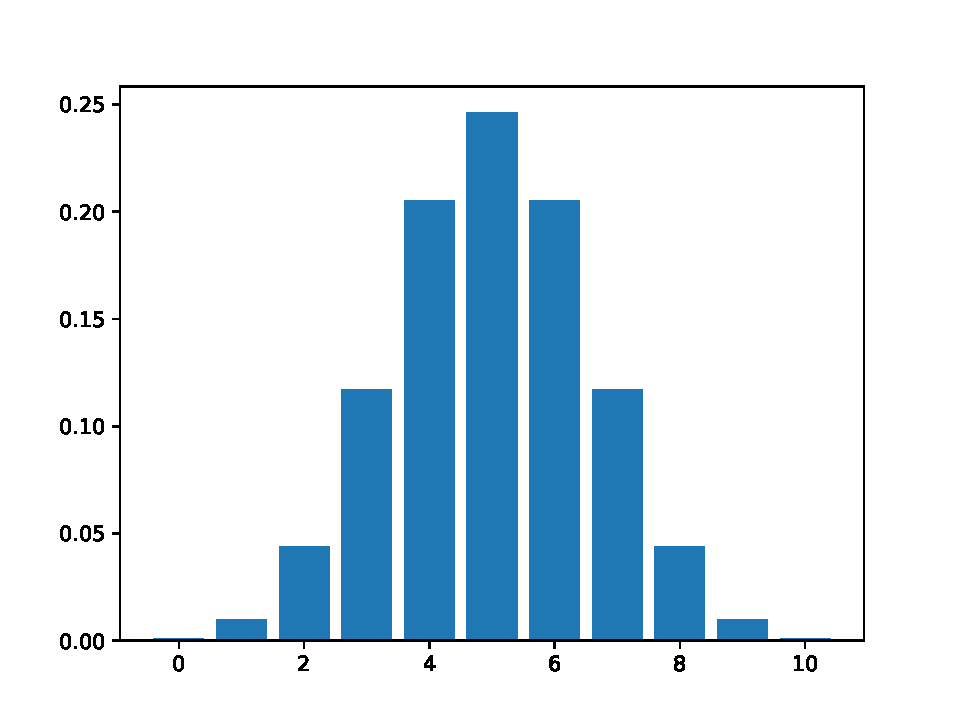
\includegraphics[width=7cm]{Figures/histogram.pdf}
%   \caption{probability with 10 periods}
%   \end{minipage}
%   \begin{minipage}[t]{0.5\textwidth}
%   \centering
%   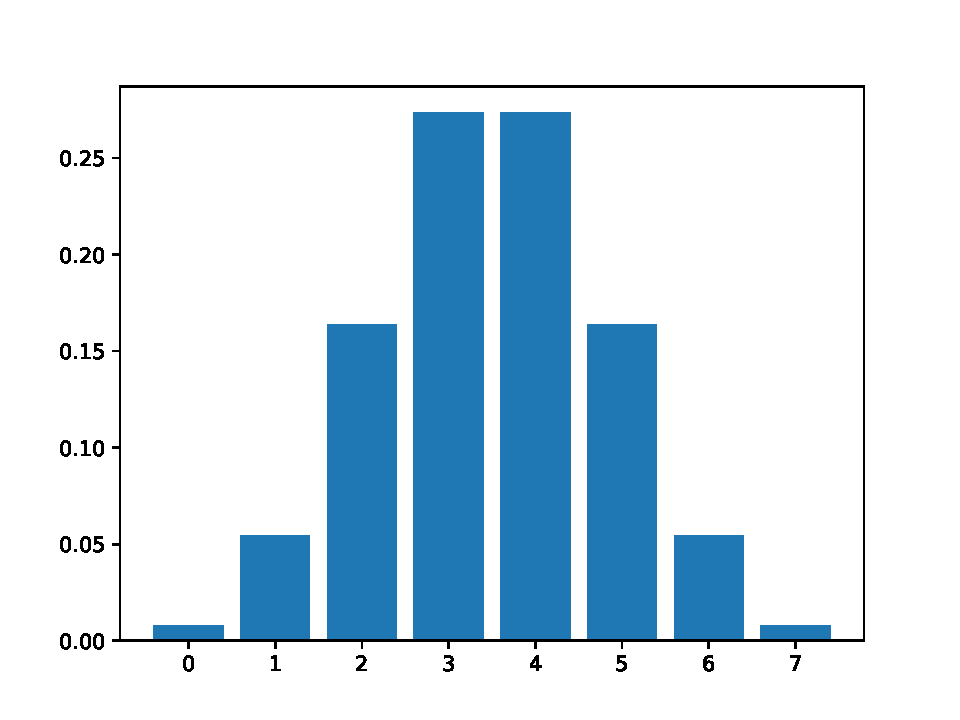
\includegraphics[width=7cm]{Figures/histogram1.pdf}
%   \caption{probability with 7 periods}
%   \end{minipage}
% \end{figure}

% Suppose that we obtain a solution, $[3,3]$, from the stochastic programming. There are $10$ periods.

% After three groups with $2$ or $3$ arrive, let us say, $2,2,2$, we need to re-calculate the probability with $7$ periods. Then we obtain $[3,3]$, when $P(D_{3} \geq 3) > \frac{1}{2}$ we will reject the groups with $2$.


% It is obvious that when the number of periods is small, we will not reject $2$ if groups with $2$ continue to arrive.

% Then, if we fix the seat assignment as $[3,3]$. For the sequence, $2,2,2,2,2,3,3,3,3,3$, we will place one $2$ in a three-seat. 
% But for the sequence, $3,3,3,3,3,2,2,2,2,2$, we will accept three $3$ and three $2$.

Show the complexity: the number of different sequences $J^{T}$, and the number of scenarios is $O(T^{J-1})$(obtained by DP).

Use $D(T,J) $ to denote the number of scenarios, which equals to the number of different solutions to $x_{1}+\ldots + x_{J} = T, \mathbf{x} \geq 0$.
Then we know the recursion relation $D(T, J) = \sum_{i= 0}^{T} D(i, J-1)$ and $D(i,2) = i+1, D(i,1) = 1$.
$D(T,3) = \frac{(T+2)(T+1)}{2}, D(T,J) = O(T^{J-1})$.

The number of scenarios is too large to enumerate all possible cases.
Thus, we choose to sample some sequences from the multinomial distribution.

Example:
The group types are $[2,3,4,5]$. The number of periods is $20$. The number of given rows is 4 and the number of seats is 22.
Each group arrives with the same probability.
The number of sequences generating from multinomial distribution is $1000$. Then, we can obtain $[0,3,6,11]$ from stochastic programming. 

When the number of sequences is 5000, we still obtain $[0,3,6,11]$. It shows that sampling is practical.

Because every period is independent, re-calculating scenarios and associated probabilities seems unimportant.

What matters is how we deal with the small-size group.

Recall that the stochastic programming only considers the situation that small-size groups can use the surplus large-size seats.

If we encounter a scenario $[5,5,5,5]$, we need to decide whether to put the small-size group into larger seats.
% (For this case, it is easy to determine because groups arrive at each period.)

If the supply is $[0,3,6,11]$, then here comes a group of 1. There will be three choices.
\begin{align*}
1 \geq 2 P(D_{2} & \geq x_{2}) \\
1 + 1\cdot P(D_{1}\geq 1) & \geq 3 P(D_{3}\geq x_{3}) \\
1 + 2\cdot P(D_{2}\geq (1+ x_{2})) & \geq 4 P(D_{4}\geq x_{4})
\end{align*}
$\mathbf{x}$ is the remaining supply right now.

Here is the problem, how do we deal with the probability?

Let $d(i,j)$ be the difference between acceptance and rejection on group $i$ for $j$-size seat.

Then $d(i,j) = i + (j-i-1)P(D_{j-i-1} \geq x_{j-i-1}+1) - j P(D_{j} \geq x_{j}), j >i$.

To ensure optimality, we need to follow some rules:

1. When there are enough supplies, we will accept them directly.

2. The demand can be accepted by a larger-size supply when there is not enough corresponding-size supply. 

3. The demand can only be satisfied by one larger-size supply.

One intuitive decision is to choose the largest difference.

We can obtain $d(i,j) = j P(D_{j} \leq x_{j} -1) - (j-i-1)P(D_{j-i-1} \leq x_{j-i-1}) -1$ after reformulating. 
Let $F_{j}(x;T)$ be the cumulative distribution function of the number of arrival groups $D_{j}$ in $T$ periods. Then $F_{j}(x; T_{r}) = P(D_{j} \leq x)$, and $D_{j}$ follows a binomial distribution $B(T_{r}, p_{j})$, where $T_{r}$ is the numebr of remaining periods.

Thus, we only need to calculate $j F_{j}(x_{j}-1; T) - (j-i-1) F_{j-i-1}(x_{j-i-1}; T)$.

For all $j >i$, find the largest $d(i,j)$, denoted as $d(i,j^{*})$.

If $d(i,j^{*}) >0$, we will place group $i$ in $j^{*}$-size seat.

\begin{algorithm}[H]\label{several_class}
  \caption{Nested policy under fixed supply}
  \begin{description}
    \item[Step 1.] Obtain a supply, $\X^{0} = [x_1,\ldots,x_{J}]$, from the stochastic programming.
    \item[Step 2.] For the arrival group type $i$ at period $T{'}$, if $x_{i} > 0$, accept it. Let $x_{i} = x_{i} -1$. Go to step 4.
    \item[Step 3.] If $x_{i} = 0$, find $d(i,j^{*})$. If $d(i,j^{*})>0$, accpect group type $i$. Set $x_{j^{*}} = x_{j^{*}} -1$. Let $x_{j-i-1} = x_{j-i-1} + 1$ when $j-i-1>0$. If $d(i,j^{*}) \leq 0$, reject group type $i$.
    \item[Step 4.] If $T{'} \leq T$, move to next period, set $T{'} = T{'}+1$, go to step 2.
  \end{description}
\end{algorithm}

\subsection{Result}

\begin{table}[ht]
  \begin{tabular}{l|l|l|l}
  \hline
  Offline & greedy & one stochastic & several stochastic \\
    & 4  & 1 & 0 \\
    & 4  & 3 & 0 \\
    & 4  & 4 & 2  \\
    & 4  & 5 & 1 \\
    & 4  & 7 & 3  \\
    & 4  & 5 & 1  \\
    & 4  & 1 & 0  \\
    & 4  & 1 & 0 \\
    & 4  & 1 & 0 \\
  \hline
  \end{tabular}
\end{table}

The number in table is the 

% The nested structure makes the greedy method useful.
% Remark: Similar to what we mentioned, the greedy method refers to using the largest groups to fill the seats.

Merit: The plan will be always feasible.

Demerit: Cannot cover all possible demands.

Improvement:
For $\X^{0}$, we introduce one empty seat, $x_1$. But it cannot provide the feasibility.

\subsubsection{How to generate scenario demands}
It is challenging to consider all the possible realizations; thus, it is practicable to use discrete distributions with a finite number of scenarios to approximate the random demands. This procedure is often called scenario generation.

Some papers consider obtaining a set of scenarios that realistically represents the distributions of the random parameters but is not too large. \cite{feng2013scenario} \cite{casey2005scenario}
\cite{henrion2018problem}

Another process to reduce the calculation is called scenario reduction. It tries to approximate the original scenario set with a smaller subset that retains essential features.

Solving the deterministic formulation with a large set of scenarios is not tricky in our case.

For the stochastic situation, we assume the group sizes are discretized from independent random variables following some distribution.(non-negative)

Every time we can regenerate the scenario based on the realized demands. (Use the conditional distribution or the truncated distribution)

If we need to assign seats before the groups' arrival, we can select any planning supply and fix it. 

If we don't need to assign seats immediately, we can wait until all demands are realized. During the process, we only need to decide whether to reject or accept each request.

Suppose that the groups arrive from small to large according to their size. Once a larger group comes, the smaller one will never appear again.

When a new group arrives (suppose we have accepted $n$ groups with the same size), we accept or reject it according to the supply (when $n+1 < \text{supply}$, we accept it), then update the scenario set according to the truncated distribution. We can obtain a new supply with the new probability and scenario set.

With the conclusion of section \ref{sec_adjacent}, we know how to reject a request. Once we reject one group, we will reject all groups of the same size. 

Fix the supply of this group size, and continue this procedure.  

If groups arrive randomly, the procedure will be similar. 

We don't care about the arrival sequence; only the number of groups matters. Because as long as the approximation about the number of groups is accurate, we can handle any sequence.

\subsubsection{Revised model}

In view of the fact that IP of the deterministic model can be solved quickly, the column generation method does not show an obvious advantage. We can revise the stochastic model as follows:

\begin{equation}\label{revised_form}
  \begin{aligned}
  \max \quad & E_{\omega}\left[\sum_{i=1}^{m-1} (s_i-1) (\sum_{j= 1}^{N} x_{ij} + y_{i+1,\omega}^{+} - y_{i \omega}^{+}) + (s_m-1) (\sum_{j= 1}^{N} x_{mj} - y_{m \omega}^{+})\right] \\
  \text {s.t.} \quad & \sum_{j= 1}^{N} x_{ij}-y_{i \omega}^{+}+
  y_{i+1, \omega}^{+} + y_{i \omega}^{-}=d_{i \omega}, \quad i =1,\ldots,m-1, \omega \in \Omega \\
  & \sum_{j= 1}^{N} x_{ij} -y_{i \omega}^{+}+y_{i \omega}^{-}=d_{i \omega}, \quad i = m, \omega \in \Omega \\
  & \sum_{i=1}^{m} s_{i} x_{ij} \leq L_j, j =1,\ldots, N\\
  & y_{i \omega}^{+}, y_{i \omega}^{-} \in \mathbb{Z}_{+}, \quad i \in I, \omega \in \Omega \\
  & x_{ij} \in \mathbb{Z}_{+}, \quad i=1,\ldots,m, j =1,\ldots,N.
  \end{aligned}
\end{equation}

After decomposition, we can obtain the master problem,

\begin{equation}\label{BD_revised}
  \begin{aligned}
    \max \quad & c{'} x + \sum_{\omega \in \Omega} p_{\omega} z_{\omega} \\
    \text {s.t.} \quad & \sum_{i = 1}^{m} s_i x_{ij} \leq L_{j}, j=1,\ldots,N \\
    & (\alpha^{j}){'}(\mathbf{d}_{i,\omega}- \sum_{j=1}^{N} x_{ij}) \geq z_{\omega}, \alpha^j \in \mathcal{O}^{t}, \forall \omega \\
     & x \geq 0
  \end{aligned}
\end{equation}

The sub-problem will be the same as \eqref{BD_sub_dual}.

When the decomposition method terminates, we set $\mathbf{x}$ as the integer variables.

The running times of solving IP directly and using Benders decomposition are shown in the table below. I list the running time of solving IP after Benders decomposition seperately to show the feasibility.

\begin{table}[ht]
  \begin{tabular}{l|l|l|l|l}
  \hline
  \# of Scenarios & running time of IP(s) & Benders \& IP(s) & \# of rows & \# of groups \\
  1000  & 5.1  & 0.13, 0.016 & 30 & 8 \\
  5000  & 28.73 & 0.47, 0.012 & 30 & 8 \\
  10000 & 66.81  & 0.91, 0.022 & 30 & 8 \\
  50000 & 925.17 & 4.3, 0.044 & 30 & 8 \\
  \hline
  1000  & 5.88 & 0.29, 0.098 & 200 & 8 \\
  5000  & 30.0 & 0.62, 0.078 & 200 & 8 \\
  10000 & 64.41 & 1.09, 0.081 & 200 & 8 \\
  50000 & 365.57 & 4.56, 0.091 & 200 & 8 \\
  \hline
  1000  & 17.15  & 0.18, 0.024 & 30 & 16  \\
  5000  & 105.2  & 0.67, 0.026 & 30 & 16  \\
  10000 & 260.88 & 1.28, 0.028 & 30 & 16  \\
  50000 & 3873.16 & 6.18, 0.05  & 30 & 16  \\
  \hline
  \end{tabular}
\end{table}


The parameters of the first experiment:
The number of rows is 30.
The number of groups is 8.
The number of seats for each row L is generated from (21, 50) randomly, about 1000 seats.
The scenarios of demands are generated from (150, 350) randomly.


The parameters of the second experiment:
The number of rows is 200.
The number of groups is 8.
The number of seats for each row L is generated from (21, 50) randomly, about 7000 seats.
Demands: (1000, 2000)


The parameters of the third experiment:
The number of rows is 30.
The number of groups is 16.
The number of seats for each row L is generated from 41-60 randomly, about 1500 seats.
The scenarios of demands are generated from (150, 250) randomly.

Fix the number of seats for each row and the number of scenarios, consider the effect of different scenarios of demands. Fix the number of scenarios at 5000.

Considering the scenarios 

\begin{table}[ht]
  \begin{tabular}{l|l|l|l|l}
  \hline
  Scenarios of demands & running time of IP(s) & Benders \& IP(s) & \# of rows & \# of groups \\
  (25,30)  & 106.71 & 92.04, 54.732 & 30 & 8 \\
  (20,40)  & 318.91 & 243.4, 219.975 & 30 & 8 \\
  (10,60)  & 48.42  & 96.98, 83.701 & 30 & 8 \\
  (10,100) & 38.41  & 38.86, 29.874 & 30 & 8 \\
  \hline
  (100,200) & 69.07 & 243.5, 156.618 & 200 & 8 \\
  (100,300) & 57.86 & 394.49, 346.657 & 200 & 8 \\
  (50,250) & 72.11  & 717.53, 642.289 & 200 & 8 \\
  (50,150) & 124.11  & 594.15, 562.371 & 100 & 8 \\
  \hline
  (5,15)   & 138.94  & 197.41, 131.32 & 30 & 16  \\
  (10,20)  & 1466.73 & 444.67, 420.034 & 30 & 16  \\
  (10,30)  & 258.56 & 78.72, 62.136 & 30 & 16  \\
  (25,30)  & 96.4  & 8.05, 1.094 & 30 & 16  \\
  \hline
  \end{tabular}
\end{table}

Three problems:
1. When the seats are larger than the number of people, Benders decomposition will give a solution like $[***,0,0,0]$.
2. In fact, we cannot obtain the optimal integral solution by using Benders and IP. That is because it relaxes more constraints.
3. When we add more constraints, the Benders shows something wrong.

\begin{equation}\label{BD_demands}
  \begin{aligned}
    \max \quad & c{'} x + \sum_{\omega \in \Omega} p_{\omega} z_{\omega} \\
    \text {s.t.} \quad & \sum_{i = 1}^{m} s_i x_{ij} \leq L_{j}, j=1,\ldots,N \\
    & \sum_{j =1}^{N} x_{ij} \geq d_{i}^{a}, i=1,\ldots,m \\
    & (\alpha^{j}){'}(\mathbf{d}_{i,\omega}- \sum_{j=1}^{N} x_{ij}) \geq z_{\omega}, \alpha^j \in \mathcal{O}^{t}, \forall \omega \\
     & x \geq 0
  \end{aligned}
\end{equation}

$d_{i}^{a}$ is the number of group $i$ we have accepted when we do several stochastic programmings.

But the programming doesnot work well unless the demands are larger than supply.

\begin{table}[ht]
  \begin{tabular}{l|l|l|l|l|l}
  \hline
  \# of samples & T & prob & \# of rows & \# of groups & \# of people served (once, several) \\
  1000  & 100 & (0.4,0.4,0.1,0.1) & 7 & 4 & (272,277) \\
  1000  & 150 & (0.4,0.4,0.1,0.1) & 7 & 4 & (280,*)\\
  5000  & 150 & (0.4,0.4,0.1,0.1) & 7 & 4 & (320,*)\\
  5000  & 100 & (0.4,0.4,0.1,0.1) & 7 & 4 & (263,266)\\
  \hline
  1000  & 100 & (0.25,0.25,0.25,0.25) & 7 & 4 & (279,*)\\
  1000  & 150 & (0.25,0.25,0.25,0.25) & 7 & 4 & (293,*)\\
  5000  & 150 & (0.25,0.25,0.25,0.25) & 7 & 4 & (310,*)\\
  5000  & 100 & (0.25,0.25,0.25,0.25) & 7 & 4 & (252,*)\\
  \hline
  \end{tabular}
\end{table}

\subsubsection{Measurement}

Suppose a real scenario with a fixed sequence, $s^{r}$. Solving the following program can obtain the optimal value, $V_{s^{r}}$. (Offline)

\begin{equation*}
\begin{aligned}
  \mbox{max}\quad & \sum_{k=1}^K(\sum_{i=1}^m (s_i-1)t_i^k) x_{k} \\
  \mbox{s.t.} \quad & \sum_{k=1}^K x_{k} \leq N \\
  & \sum_{k=1}^K t_i^k x_k \leq d_i,\quad i=1,\ldots,m \\
  & x_{k} \geq 0, \quad k = 1,\ldots,K \notag
\end{aligned}
\end{equation*}

Then the difference is $V_{s^{r}} - \text{our result}$

WS(the value under wait-and-see policy with all possible scenarios)

EVPI(Expected Value of Perfect Information) = WS - the value of deterministic equivalent form


\subsubsection{How to use the stochastic demand to solve the dynamic situation?}

\cite{bent2004scenario} this paper connects the stochastic and dynamic VRP.


\subsection{The Property}
In view of the complexity and uncertainty of branch scheme, we should analyze the property of this problem and use it to obtain a solution.

At first, we consider the types of pattern. For each pattern $k$, we use $\alpha_k, \beta_k$ to indicate the number of groups and the left space, respectively. Denote $(\alpha_k + \beta_k)$ as the loss for pattern k, $l(k)$.
% Notice that the left space is the true loss.

% When $l(k)$ reaches minimum, the corresponding pattern $k$ is the optimal solution for a single row of seats.

Let $I_1$ be the set of patterns with the minimal loss. Then we call the patterns from $I_1$ are largest. And the pattern with zero left space is called full pattern.
% Notice that a pattern from $I_1$ may not be full.
Recall that we use the vector $(t_1,t_2,\ldots,t_m)$ to represent a pattern, where $t_i$ is the size of group $i$. For example, take the length of each row be $S = 21$, the size of group types be $s = [2,3,4,5]$. Thus these patterns, $(5,5,5,5,1),(5,4,4,4,4),(5,5,5,3,3)$, belongs to $I_1$. Notice that the pattern, $(0,0,0,4)$, is not full because there is one left space.

Now consider this special case, $[2,3,\ldots,u]$, the group sizes are consecutive integers starting from 2. Then we can use the following greedy way to generate the largest pattern. Select the maximal group size,$u$, as many as possible and the left space is occupied by the group with the corresponding size. The loss is $q+1$, where $q$ is the number of times $u$ selected. Let $S = u\cdot q + r$, when $r>0$, we will have at least $\lfloor \frac{r+u}{2} \rfloor -r +1$ largest patterns with the same loss. When $r =0$, we have only one possible largest pattern.

\begin{lem}
If all patterns from an integral feasible solution belong to $I_1$, then this solution is optimal.
\end{lem}

This lemma holds because we cannot find a better solution occupying more space.

When the number of given rows is small, we can construct a solution in the following way. Every time we can select one pattern from $I_1$, then minus the corresponding number of group type from demand and update demand. Repeat this procedure until we cannot generate a largest pattern. Compare the number of generated patterns with the number of rows. If the number of rows is small, this method is useful.

\begin{corollary}
When the left updated demand can form a largest pattern, the optimal solution is the combination of patterns from $I_1$.
\end{corollary}

For example, when given the demand $d = (10,11,12,10)$ and three rows.
By column generation, we will obtain the solution $2.333 \times (0,0,0,4)_d, 0.667 \times (0,0,4,1)_d$. But we can construct an integral solution $2 \times (0,0,0,4)_d, 1 \times (0,1,2,2)_d$ or $3 \times (0,0,4,1)_d$, that depends on which pattern we choose at the beginning.

But how could we know if the number of rows is small enough?
We can consider the relation between the demand and the number of group types in patterns. Then we develop the following theorem:
\begin{thm}\label{I_1}
  When $N \leq \max_{k\in I_1} \min_{i} \{\lfloor \frac{d_i}{b_i^k}\rfloor\}$, select $k^*$-th pattern from $I_1$ and it is the optimal solution.
  $N$ is the number of rows, $i = 1,2,\ldots, m$, $d_m$ is the demand of the largest size, $b_m^k$ is the number of group $m$ placed in pattern $k$.
\end{thm}

In the light of the Theorem \ref{I_1}, when the number of given rows is small, we just need to select some patterns from $I_1$.
Continuing with the above example, we just take $(5,5,5,5), (5,4,4,4,4), (5,5,4,4,3)$ as the alternative patterns. For each $k$, $\min_{i} \{\lfloor \frac{d_i}{b_i^k}\rfloor\}$ will be $2,3,5$ respectively. So when $N \leq 5$, we can always select the pattern $(5,5,4,4,3)$ five times as the optimal solution.

When column generation method gives an integer solution at the first time, we obtain the optimal solution immediately. Now suppose that we have a fractional solution. Divide the solution into a pure integral part and the fractional part. The fractional solution will have a corresponding integral supply occupying the same space size. When the rest groups can be placed in the rest rows(given rows minus the integral rows), then the total groups can be placed in the given rows.

% \begin{lem}
% If the patterns obtained by column generation are all full, the total groups can be placed in the given rows if and only if the rest groups can be placed in the rest rows.
% \end{lem}
%
% The necessity is clear. For the sufficiency, this is because the space occupied by the integral supply is fixed, and the capacity of the supply corresponding to the integral pattern cannot be improved.(They are all full.)

Based on the above analysis, we can establish an algorithm below.

\begin{algorithm}[H]\label{algoDI}
\caption{Optimal solution to seat assginment problem with fixed demand}
\begin{description}
  \item[Step 1.] Obtain the solution from \eqref{lambda1}. If the solution is integral, terminate this algorithm. Then, for the fractional solution $x{'}$, calculate the supply quantity $q{'}=(q_1,\ldots,q_m) = Tx{'}$ for each group type. If each element is integral, go to step 3. If any element of this supply is not integral, go to step 2 to construct an integer supply vector which can provide the largest integral profit.
  \vspace{5pt}
  \item[Step 2.] Construction: calculate the space occupied by fractional supply and the corresponding profit. The size of space must be integral. Increase the corresponding-size supply by 1, then delete the fractional part. If the size of space is 1, delete the corresponding fractional part directly. 
  % If the space occupied by fractional supply is fractional, find the supply providing the same profit according to the greedy rule.

  \item[Step 3.] Take this integral supply vector $q$ as a new demand and obtain a new LP solution $x^{*}$ with column generation. Divide $x^{*}$ into a pure integral part $x^I$ and fractional part $x^F$. Subtract the corresponding supply of the integral part $x^I$ from the new demand $q$ to obtain the rest groups($r = q - q^I$). $N$ is the number of given rows. The number of rest rows equals to $N - \sum x^I$.
  \item[Step 4.] Use subset sum problem to check if the rest groups can be placed in rest rows.
  \item[Step 5.] If the rest groups can be placed, then we find an optimal solution. If the rest cannot be placed, find a new supply providing the maximal people without exceeding the capacity and go to step 2 to construct a new supply.
\end{description}
\end{algorithm}

Summary:
Two main procedures: 1. From the fractional solution(fractional supply) to intergal supply(according to the nature of our problem, i.e., we have the upper bound of elements of supply)  step 1.2.
2. From integral supply to integral pattern.(Check the feasibility)  step 3.4.

Reason of construction:

\begin{thm}
  The supply obtained from (2) has at most one fractional element.
\end{thm}

Notice that from (2), we have an upper bound of demand, and the larger-size group has more people per seat on average.

% Thus, the linear result must place groups from big to small according to their size.

To show it by contradiction. Now we obtain a supply, $[q_1, q_2, \ldots, q_{J}]$, find the first fractional element from $q_{J}$ to $q_{1}$, let it be $q_{m}$. There exists a non-zero number among $q_{j}, j<m$. Then increasing $q_{m}$ by $\alpha$ to $\lceil q_{m} \rceil$ from the seats taken by $q_{j}$ can give a higher objective value, i.e., $\alpha m > \frac{\alpha(m+1)}{j+1} j$. Follow this procedure until at most one fractional value among $q_1, q_2, \ldots, q_{J}$. 
And when $q_i$ is the fractional number, all $q_k, k<i =0$. With the constraint that the supply should be no larger than the demand, $q_k = d_k, k>i$.

Thus, we will only have the supply with at most one fractional element.

\begin{corollary}
 The solution associated with the integral supply obtained by the above procedure is an optimal integral solution to (2).
\end{corollary}

Firstly, the integral supply constructed from step 2 is a potential optimal integral supply. We still need check its feasibility, once we find a seat assignment, that is an optimal solution. If not, find a new supply providing the maximal people without exceeding the capacity, then continue to check its feasibility.

This procedure can be realized by the result of subset sum problem.


% Construction:what we need to do is to construct an integer supply, then to test if there exists a plan to accommodate these groups.

% Now we need to judge whether we need to tackle step 4 in some cases.

% For the case $(2,3,\ldots,u)$, if the rest space is 1, we can discard $1$ or exchange $1$ and $3$ with two $2$. Remember what we need to do is to construct a maxmimal integer supply.

% Assume that the demand is large such that the given rows cannot accommodate it and the number of group containing 2 people is large.

% When the demand is large, i.e. supply cannot cover the whole demand. The equation $\sum_{k \in K}^K x_{k} \leq N$ will be always valid. The sum of all elements of the solution vector always equals to the given number of rows.

% Then the rest space for each maximal pattern will be no more than 1 with the extra groups with the size of 2.

% \begin{thm}\label{full}
% For the case $(2,3,\ldots,u)$, there exist patterns to contain the rest groups.
% \end{thm}

We have a counterexample, [4,6,9,10] * [1,2,1,1], L= 18 for the original cutting plane problem. Still need to check whether the rest can construct 18.

But if we add more groups, like [2, 3, 4, 5, 6,7 ,8 ,9,10] * [1, 1, 2, 3, 2, 2, 2,1,1], we can find a seat assignment.

% We can use the induction to construct the pattern.
% When the sum of all elements of the fractional solution is 1, it is clear that the rest group will form a pattern because the summation of space occupied by the rest group will be no more than the length of row.
% When the sum is 2, suppose the rest groups cannot form a full pattern, the maximal pattern will have a left space. So there will be two rows with one unoccupied space, and we know in this situation there will be a left group with size of 1. When there are two adjacent numbers in the two patterns separately, we can change their position to accommodate these groups. As for the situation
% without adjacent numbers, it will be removed during the calculation of column generation.
% % Because we will not obtain the fractional solution for these cases.
% For example, we have 6 seats for a row. The rest groups are [2,1,1](number)* [2,3,5](size).
%
% % Once we construct the supply correctly, it will be ...
%
% When the sum is 3, if we can form a full pattern for a row, this situation converts to the situation where the sum is 2.
% Then we suppose that the left group should have the size of 3 and the three rows all contains one occupied space. But this situation will contradict with the results of column generation method.

% There are several points to consider:
%
% 2. And whether the pattern is full or not. When all pattern obtained by column generation, can we say that we definitely have the results.

% 3. For the case [2,3,4,5], we can be sure that there will be the solution to contain the rest group.


% 2) Possible extension to group sizes [a,b,c]. It is not true for any a,b,c,L. Howover, can you identify some conditions under which your idea can be applied, e.g., (2,3,7,41), (3,5,7,44)?
%
% 3) Possible extension to 4 sizes [a,b,c,d] and specific L
%
% 4) For cases that cannot be solved by your idea, can you bound the error of your idea?

% One observation is that as long as we can satisfy the largest $[d_a, d_b, d_c]$ under some policy, we can obtain an optimal solution. Can the greedy method help us to realize that?

% Because we cannot generate the largest pattern, either $D_4-d_4$ or $D_5-d_5$ will be small.
\newpage

\subsection{Definitions And Policy}

In this section, we discuss about the cases where the group size is no more than 5, we can use the greedy way to generate one largest pattern. Through this pattern, we can obtain all other largest patterns. Then we define the priority of different largest patterns. The priority may depends on the initial demands in some case and does not depend on the demands in other cases. Then we give the policy to obtain one optimal assignment. Notice that only given the specific case, we have the corresponding priority in the policy. But we give the conclusions in the following subsections.

\begin{definition}
Let $P_N = \{2,\ldots,N\}$ denote the assignment problem with up to N sizes in each group, $3 \leq N \leq 5$.
% Without loss of generality, suppose that the group sizes are consecutive integers starting from 2.
% Let $[a_1,a_2,\ldots,a_i], a_1<a_2<\ldots<a_i$ denote the group sizes.

Let $D = (d_{2},d_{3}, \ldots, d_{N})_D$ denote the initial demands of the group sizes.
\end{definition}

Recall that a feasible assignment for one row is called a pattern, which can be expressed in a compact form or an expanded form.

Compact form: Use $(p_2,p_3,\ldots,p_N)$ denote the number of group sizes in one pattern.

Expanded form : Denote by $(a,b,\ldots,d), a \geq b \geq \ldots \geq d$ the pattern, which means that the groups with the size of $a,b, \ldots, d$ are placed in a row.


For the group sizes $[a_1,\ldots,a_i], 2 \leq a_1<\ldots<a_i \leq 5, 2 \leq i \leq 4$, we have the following conclusions.

Suppose the demands are large enough, we consider a greedy way to generate a pattern.

\begin{definition}
We obtain the pattern without considering the effect of demands. The greedy way to generate a pattern is described as follows.
For any row, we will place the groups with the largest size as many as possible, then place the group whose size equals the number of the remaining seats. Because we don't consider the effect of demands, the remaining seats will be less than $2$. When the number of remaining seat is $1$ or $0$, we stop placing. In this way, we generate a greedy pattern.
\end{definition}

\begin{lem}\label{largest}
The pattern generated in the greedy way is one of the largest patterns.
\end{lem}

\begin{pf}[Proof of lemma \ref{largest}]
For each pattern $k \in I$(denote by $I$ all feasible patterns), we have two parts of loss. The first one results from the social distance between adjacent groups, we use $\alpha(k)$ to express its value. The second one is the empty seats which are not taken by any groups, use $\beta(k)$ to express its value.

The largest patterns have the minimal loss. We need to prove the greedy pattern will also have the minimal loss.

Notice that the number of remaining seats will be less than 2. Denote by $g \in I$ the greedy pattern. By placing the group with the largest size as many as possible, the pattern will have the minimal $\alpha(g)$, $\alpha(g) \leq \alpha(k), k \in I$. When the number of remaining seat is $0$, $\beta(g)$ will be 0. In these cases, the total loss will be the smallest.

When the number of remaining seat is $1$, $\beta(g)$ will be 1. Notice that any pattern $g_1$ will have at least $\alpha(g_1) = \alpha(g)+1$ when placing another group, in this way, the loss,$\alpha(g) + \beta(g) \leq \alpha(g_1)+\beta(g_1)$, will still be the smallest.
Thus, the greedy pattern is one largest pattern.
\end{pf}

\begin{lem}
Other largest patterns can be generated by the greedy largest pattern.
\end{lem}

Denote by $r$ the number of remaining seats after placing the groups with the largest size as many as possible in a row. We can generate a new largest pattern by decreasing the group with the largest size and increasing the group with the size of $r$. We can obtain all the largest patterns until the gap between the size of all placed groups is less than 2.

For example, when $S=21$, group sizes are $[2,3,4,5]$. The greedy pattern is $(5,5,5,5,1)$, which can develop the second largest pattern $(5,5,5,4,2)$, the third one $(5,5,5,3,3)$, the fourth one $(5,5,4,4,3)$, the fifth one $(5,4,4,4,4)$. Because the gap between $4$ and $5$ is 1 less than 2, we cannot decrease the largest group size and increase the smallest group size to generate another different pattern. Until here, we have obtained all the largest patterns.

\begin{remark}
$r=1$ leads to the maximum number of different largest patterns. Thus, the case, $r=1$, is the most complex part we need to consider.
\end{remark}

Our policy is to use the largest patterns as many as possible, then place the group with the largest remaining size in a greedy way. The core problem is how to obtain the maximum number of the largest patterns with the given certain demands. But maybe we have several largest patterns, and their priority will affect the maximum number of largest patterns when given the demands. Once we can determine their priority, then use the specific largest patterns according to their priority, we can obtain an optimal assignment for any given $n$ rows.

\begin{definition}
Given the number of seats in a row, $S$. The group sizes are $[a,b,c,d]$.
Suppose we have several largest patterns $k_i, i\in \{1,2,\ldots,l\}$. We assume that $k_i \succeq k_{j}, i, j\in \{1,2,\ldots,l\}$ which means we prefer pattern $k_i$ to $k_j$ in our policy when they are both available.
When the demands are enough to obtain pattern $k_i$, we say pattern $k_i$ is available. If some largest pattern is not available, just skip it in order of precedence.

When $k_1 \succeq k_2 \succeq \ldots \succeq k_l$ holds, we can follow this priority in our policy to obtain an optimal assignment for any demands $d_a, d_b, d_c, d_d$.
We can say that $k_i$ is preferred at least as much as $k_{i+1}, i = 1,2,\ldots, l-1$.

If the priority between $k_i$ and $k_j$ depends on the demands. Suppose that when $D_4 \leq D_3$, $k_i \succeq k_j$. We will always choose the preferred pattern $k_i$ until it is unavailable.

Here we need to talk about the existence of priority.
When given $S$ and $D$, the priority will remain unchanged.

\end{definition}

With the conclusions of the following subsections, we have Theorem \ref{OptimalAssignment}.


\begin{thm}\label{OptimalAssignment}
If the first $n$ rows are filled with full patterns by the greedy way, then the first $k$ rows of $n$ rows will be an optimal assignment when given $k$ rows, $1 \leq k \leq n$.
\end{thm}

If we follow this theorem to revise the assignment when we encounter the non-full pattern, maybe we can construct a new assignment until the patterns are all full.


% \begin{corollary}
% We can obtain an optimal assignment when given $n$ rows in our policy.
% The first $k$ rows of $n$ rows will be an optimal assignment when given $k$ rows, $1 \leq k<n$.
% \end{corollary}

\subsection{Counterexample}
Suppose that the largest pattern has the loss, $I$.

We need to construct an example like this, just consider three rows. For situation 1, one row has the loss $I$, the other two rows have the loss $I+2$. Another situation is these three rows all have the loss $I+1$. In this way, the largest pattern will not provide an optimal assignment for three rows.

In other words, if the largest pattern can destroy three second-largest pattern, we will obtain a counterexample.

Situation 1:
For the first row, $S = K + a_1 + a_2 + a_3$ with loss $I$.

Situation 2:
$S = K + a_1 + b_1 + b_2 + b_3$, $b_1 + b_2 + b_3 = a_2 + a_3$.

$S = K + a_2 + c_1 + c_2 + c_3$, $c_1 + c_2 + c_3 = a_1 + a_3$.

$S = K + a_3 + d_1 + d_2 + d_3$, $d_1 + d_2 + d_3 = a_1 + a_2$.

These three rows all have the loss $I+1$. $b_i,c_i,d_i < a_1 \leq a_2 \leq a_3, i=1,2,3$.

Then in situation 1, for the rest two rows, we cannot obtain a second largest pattern if $b_i,c_i,d_i$ cannot form the value of $a_1 + a_2 + a_3$.

For example,

$b_1 + b_2 + b_3 = a_2 + a_3$.
$c_1 + c_2 + c_3 = a_1 + a_3$.
$d_1 + d_2 + d_3 = a_1 + a_2$.

$5 + 5 + 6 = 8 + 8$.
% $5 + 5 + 4 = 7 + 7$.
% $4 + 4 + 4 = 6 + 6$.

$S = 8+8+8$, suppose we only have three 8, three 6, six 5.

For situation 1, we have $(8,8,8),(6,6,6,5),(5,5,5,5)$.
But for situation 2, we have three $(8,6,5,5)$ which is better than situation 1.

For $[2,3]$, S= 9, or 11, $(3,3,3)$ or $(3,3,3,2)$. When $d_2 \geq 3d_3$, $n \geq d_3$, $(3,2,2,2)$ will be better than $(3,3,3)$.
% d_3 =7, d_2 =12, S = 15, totally greedy is not correct, should use a full pattern.
For $[2,4]$, no counterexample here.

For $[2,5]$, no counterexample here.

For $[3,4]$, S= 3*m+4 = 16 + (m-4)*3. When $d_3 \geq m(d_4-1), d_4 \geq 4$, $n \geq d_4-1$, $(4,3,3,3,3)$ will be better than $(4,4,4,4)$, here $m=4$.

In general, the greedy way will provide a lower bound and when the number of group sizes are colse relatively, the greedy way will give an optimal assignment. The gap will be the summation of space loss for each row. If each row is occupied by a full pattern, then this assignment is optimal.

If we assume the demand of group size of 2,$d_2$, is large enough, the space loss for each row will be less than 2. Thus, the largest gap will be $(n-2)$ for n rows.


\newpage
